\documentclass[12pt,a4paper]{article}

\usepackage[utf8]{inputenc}
\usepackage[T1]{fontenc}
\usepackage{graphicx}
\usepackage{amsmath}
\usepackage[margin=2.5cm]{geometry}

\title{Face Blurring for Privacy Protection}
\author{
Team Members: \\[0.5em]
Habiba Ahmed Mohamed (ID: 20210120) \\
Ahmed Khaled Mohamed (ID: 20210016) \\
Mina Albert Saeed (ID: 20210417) \\
Bemwa Malak Gerges (ID: 20200116)
}
\date{\today}

\begin{document}

\maketitle

\begin{abstract}
This project presents a practical image processing system implemented in GNU Octave for automated facial privacy protection in digital images. The system follows a three-stage pipeline approach: preprocessing, face detection, and privacy protection. The preprocessing stage standardizes input images to 512x512 pixels and applies noise reduction using Gaussian smoothing. Face detection combines two complementary techniques: skin detection in YCbCr color space using calibrated thresholds (Cb: 77-127, Cr: 133-173) and edge detection using Sobel operators, resulting in reliable face localization for front-facing subjects in well-lit conditions.

The privacy protection mechanism implements a two-phase approach: initial pixelation followed by Gaussian blur. The pixelation block size automatically adjusts to 1/20th of the detected face dimension, ensuring appropriate privacy protection while maintaining natural appearance. All image processing operations, including color space conversion, convolution, and kernel generation, are implemented using basic mathematical operations, making the system portable and independent of specialized toolboxes. This implementation provides a straightforward solution for basic privacy protection needs while remaining accessible through the open-source Octave platform.
\end{abstract}

\section{Problem Definition and Objectives}
\subsection{Problem Statement}
The widespread sharing of digital images on social media and other platforms has created a pressing need for automated privacy protection. While manual face blurring is possible, it becomes impractical when dealing with multiple images. Many existing solutions either require expensive software licenses or rely on complex deep learning models.

This project implements a straightforward yet effective face detection and privacy protection system using GNU Octave. The solution focuses on balancing accuracy and simplicity, providing a practical tool for basic face detection and privacy protection without requiring specialized hardware or proprietary software.

\subsection{Objectives}
\begin{itemize}
    \item \textbf{Face Detection:}
    \begin{itemize}
        \item Implement a basic face detection system using color and edge information
        \item Use YCbCr color space for reliable skin tone detection
        \item Combine edge detection with skin detection for improved accuracy
        \item Handle single-face detection in well-lit, front-facing scenarios
    \end{itemize}
    
    \item \textbf{Privacy Protection:}
    \begin{itemize}
        \item Create an effective two-step privacy filter using pixelation and blur
        \item Implement adaptive blurring based on face size
        \item Ensure the protected image maintains a natural appearance
        \item Process images efficiently using basic image processing operations
    \end{itemize}
    
    \item \textbf{Implementation:}
    \begin{itemize}
        \item Develop the system using only GNU Octave's core functionality
        \item Create a simple pipeline for image preprocessing, detection, and protection
        \item Ensure code readability and maintainability
        \item Provide a practical solution for basic privacy protection needs
    \end{itemize}
\end{itemize}

\section{Methodology}
The implementation of the system follows a three-stage pipeline approach, with each stage carefully designed to handle specific aspects of the face detection and privacy protection process.

\subsection{Stage 1: Image Preprocessing}
The preprocessing stage prepares input images for face detection through three main steps: standardization, color processing, and noise reduction.

\subsubsection{Image Standardization}
Input images are resized to 512x512 pixels using nearest-neighbor interpolation.

\subsubsection{Color Channel Processing}
The RGB channels are processed separately, with each channel normalized to the uint8 range (0-255).

\subsubsection{Noise Reduction}
A 5x5 Gaussian smoothing filter with sigma=1 is applied to reduce image noise while preserving important facial features. The filter is applied to each color channel independently through convolution operations.

\subsection{Stage 2: Face Segmentation}
The face segmentation stage combines color-based skin detection with edge information to locate faces in the preprocessed image.

\subsubsection{Color Space Transformation}
The RGB image is converted to YCbCr color space to separate brightness (Y) from color information (Cb, Cr).

\subsubsection{Dual-Channel Detection}
Face detection uses two parallel processes:
1. Edge detection using Sobel operators on the luminance (Y) channel with adaptive thresholding at twice the mean magnitude.
2. Skin detection by applying thresholds to chrominance components (Cb: 77-127, Cr: 133-173).

These results are combined using a logical AND operation to create a binary mask of potential face regions.

\subsubsection{Face Region Localization}
The algorithm identifies face regions from the binary mask by computing boundary coordinates. It then creates a bounding box around the detected face area, adjusting for typical face proportions and image boundaries.

\subsubsection{Visualization}
\begin{figure}[h]
    \centering
    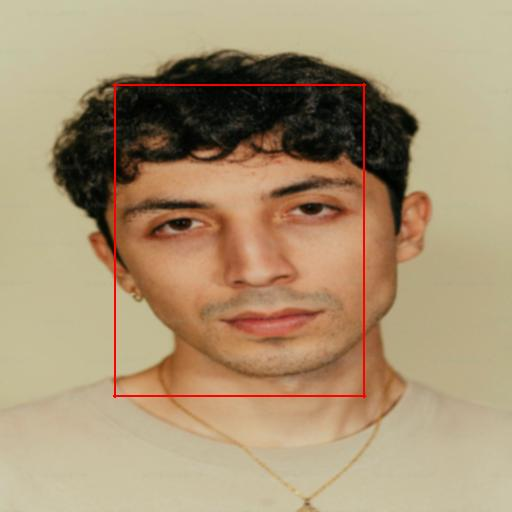
\includegraphics[width=0.4\textwidth]{sample_image.jpg}
    \caption{A segmented image after face detection}
    \label{fig:segmented_image}
\end{figure}

\subsection{Stage 3: Face Privacy Protection}
The final stage applies privacy protection by blurring the detected face region through a two-step process.

\subsubsection{Region Processing}
The detected face region is first extracted using the bounding box coordinates. The blurring intensity is automatically adjusted based on face size, with the block size set to 1/20th of the smallest face dimension to ensure appropriate privacy protection.

\subsubsection{Privacy Filter Application}
The privacy filter combines pixelation and Gaussian blur:
1. The face region is divided into blocks, with each block's color averaged to create a pixelation effect
2. A 3x3 Gaussian filter smooths the pixelated regions to produce a more natural appearance

\begin{figure}[h]
    \centering
    \includegraphics[width=0.4\textwidth]{sample_image(blurred).jpg}
    \caption{Result of privacy protection}
    \label{fig:privacy_protection}
\end{figure}

\end{document}